\documentclass[journal=jacsat,manuscript=article]{achemso}

\usepackage[version=3]{mhchem} % Formula subscripts using \ce{}

\usepackage{xcolor,soul}
\setlength\marginparwidth{1.5cm}
\usepackage[obeyFinal,textsize=tiny, textwidth=\marginparwidth]{todonotes}
\presetkeys{todonotes}{fancyline, color=blue!30}{}

%%%%%%%%%%%%%%%%%%%%%%%%%%%%%%%%%%%%%%%%%%%%%%%%%%%%%%%%%%%%%%%%%%%%%
%% If issues arise when submitting your manuscript, you may want to
%% un-comment the next line.  This provides information on the
%% version of every file you have used.
%%%%%%%%%%%%%%%%%%%%%%%%%%%%%%%%%%%%%%%%%%%%%%%%%%%%%%%%%%%%%%%%%%%%%
%%\listfiles

%%%%%%%%%%%%%%%%%%%%%%%%%%%%%%%%%%%%%%%%%%%%%%%%%%%%%%%%%%%%%%%%%%%%%
%% Meta-data block
%% ---------------
%% Each author should be given as a separate \author command.
%%
%% Corresponding authors should have an e-mail given after the author
%% name as an \email command. Phone and fax numbers can be given
%% using \phone and \fax, respectively; this information is optional.
%%
%% The affiliation of authors is given after the authors; each
%% \affiliation command applies to all preceding authors not already
%% assigned an affiliation.
%%
%% The affiliation takes an option argument for the short name.  This
%% will typically be something like "University of Somewhere".
%%
%% The \altaffiliation macro should be used for new address, etc.
%% On the other hand, \alsoaffiliation is used on a per author basis
%% when authors are associated with multiple institutions.
%%%%%%%%%%%%%%%%%%%%%%%%%%%%%%%%%%%%%%%%%%%%%%%%%%%%%%%%%%%%%%%%%%%%%
\author{Josh J. Kirsopp}
\author{Athanasios Arvanitidis}
\author{Peter J. Knowles}
\email{KnowlesPJ@Cardiff.ac.uk}
\affiliation[Cardiff University]
{School of Chemistry, Cardiff University, Cardiff CF10 3AT, United Kingdom}


% \title[Orbital-fitted density]
%   {Approximating molecular electrostatic potentials through minimal representations of local molecular orbitals}
\title[Reduced Orbital Potential Approximation]
  {Approximating molecular electrostatic potentials: the Reduced Orbital Potential Approximation}


%\abbreviations{IR,NMR,UV}
%\keywords{American Chemical Society, \LaTeX}


\begin{document}


\begin{tocentry}

Some journals require a graphical entry for the Table of Contents.
This should be laid out ``print ready'' so that the sizing of the
text is correct.

Inside the \texttt{tocentry} environment, the font used is Helvetica
8\,pt, as required by \emph{Journal of the American Chemical
Society}.

The surrounding frame is 9\,cm by 3.5\,cm, which is the maximum
permitted for  \emph{Journal of the American Chemical Society}
graphical table of content entries. The box will not resize if the
content is too big: instead it will overflow the edge of the box.

This box and the associated title will always be printed on a
separate page at the end of the document.

\end{tocentry}


\begin{abstract}
  The abstract.
  Will define
  Distributed Multipole Analysis (DMA).
\end{abstract}


\section{Introduction}
Introduction

  Will define
  Distributed Multipole Analysis (DMA)\cite{Stone1981,Stone1985,Stone2005}.
Cite some papers\cite{Knizia2015}

\section{Theory}

For an $N$-electron molecule with electronic wavefunction $|\Psi\rangle$ the clamped-nucleus charge density is
\begin{align}
    \rho(\vec r) = \sum_A Z_A \,\delta(\vec r - \vec A)
    -N \,\langle\Psi|\delta(\vec r-\vec r_1)|\Psi\rangle
\end{align}
where $\vec A, Z_A$ denote the positions and charges of the nuclei, and
$\vec r_1$ is the coordinate of one of the electrons.
The electrostatic potential arising from this or any charge density $\rho$ is
\begin{align}
    J[\rho] &= \int d\vec r' \rho(\vec r') |\vec r-\vec r'|^{-1}
\end{align}

% The corresponding electrostatic potential is then
% \begin{align}
    % V(\vec r) & =
    % \sum_A Z_A |\vec r
    % - \vec A|^{-1}+\sum_i J[|\psi_i|^2](\vec r)
% \end{align}
In the distributed multipole approach\cite{Stone1981,Stone1985,Stone2005} a simple approximation to the potential is
obtained via  a model charge density consisting of point charges, dipole, and higher multipole, moments centred on the atoms.
The quantum-mechanical multipole operators associated with an origin $\vec A$ are\cite{Stone2013}
\begin{align}
    \hat Q_{lm}^A &= \sum_a e_a\, R_{lm}(\vec r_a-\vec A)
    \\
R_{lm}(\vec r)&=\sqrt{\frac{4\pi}{2l+1}}\,r^l \, Y_{lm}(\vec r)
,&
I_{lm}(\vec r)&=\sqrt{\frac{4\pi}{2l+1}}\,r^{-l-1} \, Y_{lm}(\vec r)
\end{align}
where
$e_a, \vec r_a$ are the charges and positions of each particle, and 
$R_{lm}, I_{lm}$ are the regular and irregular solid harmonics\cite{Whittaker1927, Stone2013}.
The potential generated by a unit-magnitude multipole  centred at $\vec A$ is
    $ (-1)^m I_{l,-m}(\vec r-\vec A)$,
% \begin{align}
    % V^A_{lm}(\vec r) = (-1)^m I_{l,-m}(\vec r-\vec A)
% \end{align}
and one assigns
%, by appropriate projection, best-fit and locality criteria
with an appropriate algorithm\cite{Stone1981,Stone1985,Stone2005}
values $\{Q^A_{lm}\}$ for the site multipole moments, leading to overall model electrostatic potential
\begin{align}
    V^{\text{DMA},L}(\vec r) &= \sum_A \sum_{lm}^L(-1)^m\, Q^A_{lm}\, I_{l,-m}(\vec r-\vec A)
\end{align}
where $L$ is the
maximum angular momentum, $0\le l\le L, -l\le m\le l$, beyond which the multipole expansion is truncated.

In this work, we investigate the possibility of assigning a site of model electronic density and associated potential with each molecular orbital, rather than nuclei (which remain in the model as point nuclear charges only).

For a molecule represented by Hartree-Fock or Kohn-Sham theory, such a model can be exact, since the density is
\begin{align}
    \rho(\vec r) = \sum_A Z_A \delta(\vec r - \vec A)
    -\sum_i |\psi_i(\vec r)|^2
\end{align}
where $\{\psi_i\}$ are the occupied molecular spin-orbitals.
However we furthermore seek a model that, for efficiency reasons, is as computationally
simple as possible, and which is also based on localised orbitals, in order
to ensure stability and uniqueness as the size of the molecule is varied. We assume
from this point forwards that $\{\psi_i\}$ denote orbitals from a Kohn-Sham
or Hartree-Fock calculation rotated using the Pipek-Mezey procedure\cite{Pipek1989a}.

\subsection{Orbital Multipole Approximation}

For each orbital, we define an origin that is its charge centroid, i.e., the
choice of origin that gives zero dipole moment for the orbital,
\begin{align}
  \vec r_i = \int d \vec r \,|\psi_i(\vec r)|^2 \,  \vec r
\end{align}
We can then compute the multipole moments arising from the orbital at this origin,
\begin{align}
    Q^i_{lm} = -\int d\vec r \, R_{lm}(\vec r-\vec r_i) \, |\psi_i|^2
    .
\end{align}
Note that by construction there is no dipole ($l=1$) contribution, and $Q^i_{00}=-1$, representing the unit occupancy of spin-orbital $\psi_i$. The first characteristic shape descriptor of the orbital is therefore its quadrupole moment.
Specification of a maximum angular momentum $L$, $0\le l\le L, -l\le m\le l$ is then sufficient to completely define an Orbital Multipole Approximation (OMA) for the potential,
\begin{align}
    V^{\text{OMA},L}(\vec r) &=
    \sum_A Z_A |\vec r
    - \vec A|^{-1}
    % +\sum_i J[|\psi_i|^2](\vec r)
    +\sum_i \sum_{lm}^L(-1)^m\, Q^i_{lm}\, I_{lm}(\vec r - \vec r_i)
    .
\end{align}
Just as with DMA, this model is expected to be faithful, with a convergent series, when evaluated at positions that are sufficiently distant from any of the nuclei or orbital centroids, but omits the
charge-penetration screening of the Coulomb interaction, and for very short $|\vec r-\vec r_i|$ or $|\vec r-\vec A|$ will give divergence. Unlike DMA, OMA is not dependent on any assumption that molecular densities are approximately the sum of near-spherical atomic densities. The localized molecular orbitals are natural centres of charge that arise automatically in the determination of the wavefunction, and there is no need for any artificial construction based
on basis-function centres\cite{Stone1981} or partitioning switch functions\cite{Stone2005}.
In Figure~\ref{fig:1}, we show the exact $V(\vec r)$, together with
$V^{\text{DMA},L}$ and
$V^{\text{OMA},L}$ for several values of $L$, and for several $\vec r$ along the molecular axis of carbon monoxide.
It is seen that, in general, both the DMA and OMA approximations provide an accurate representation of the potential outside around 1.5 van der Waals radii; however there are significant errors if the multipole expansion is truncated at second order, especially in the OMA case.
\begin{figure}
    \centering
    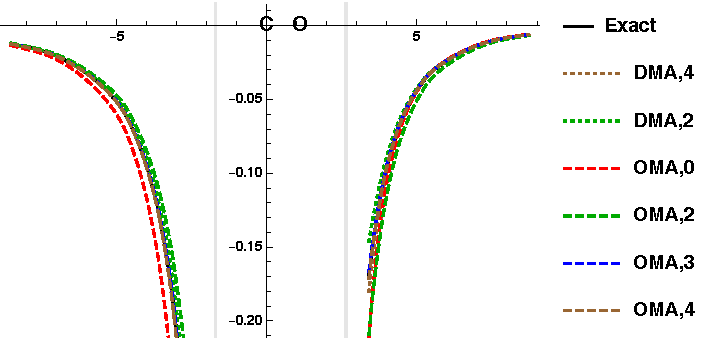
\includegraphics{fig1.pdf}
    \caption{Distributed multipole electrostatic potential / Volt at points along the molecular axis of CO arising from a B3LYP calculation with the aug-cc-pVQZ basis set\cite{Kendall1992a}. C is at the coordinate origin, and O at $(0,0,r_e=1.1282\text\AA)$.
    The van der Waals radii of the atoms\cite{Bondi1964VanRadii} ($r_C=1.70\,\text\AA$ and $r_{\text O}=1.52\,\text\AA$) are indicated in grey.
    Atom-distributed multipoles (DMA,$L$) are taken from Ref.~\citenum{Stone2005}.
    }
\label{fig:1}
\end{figure}

Figure~\ref{fig:2} shows the same data expressed as the difference from the exact $V(\vec r)$, and focusing on the low-energy asymptotic region.
\begin{figure}
    \centering
    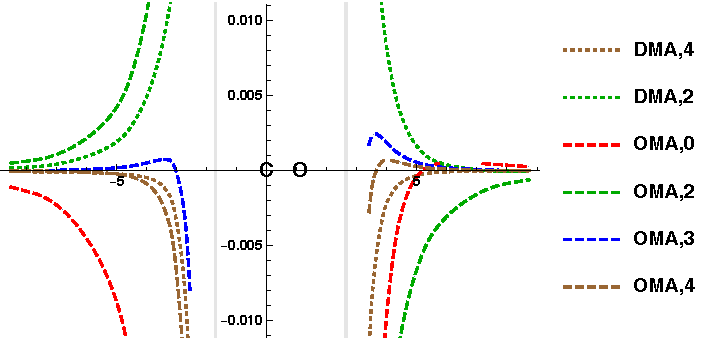
\includegraphics{fig2.pdf}
\caption{Error in distributed multipole electrostatic potential / Volt at points along the molecular axis of CO arising from a B3LYP calculation with the aug-cc-pVQZ basis set\cite{Kendall1992a}. C is at the coordinate origin, and O at $(0,0,r_e=1.1282\text\AA)$.
    The van der Waals radii of the atoms\cite{Bondi1964VanRadii} ($r_C=1.70\,\text\AA$ and $r_{\text O}=1.52\,\text\AA$) are indicated in grey.
    Atom-distributed multipoles (DMA,$L$) are taken from Ref.~\citenum{Stone2005}.
    }
    \label{fig:2}
\end{figure}
Near to oxygen, OMA,3 and OMA,4 show superior accuracy to DMA,4, with the onset of divergence occurring closer to the atom.
At the carbon end of the molecule, the situation is reversed, with DMA,4 being slightly more stable. All approximations start to diverge at a somewhat longer distance from C than from O.
For a large molecule, DMA and OMA will typically have similar numbers of multipole sites; for example, in the case of polyethene, each \ce{CH2} unit has three DMA sites; for OMA, there are three valence-orbital sites plus the core monopole, assuming, as likely, that the carbon $1s$ orbital can be approximated as a monopole centred on the nucleus.
OMA is thus promising as an alternative to DMA that is worthy of further investigation. It has the advantage that it is determined entirely by a Kohn-Sham calculation, and does not depend on the assumptions of any particular atomic partitioning scheme.

\subsection{Reduced-orbital Potential Approximation}

Any distributed multipole expansion has the advantage of a larger region of convergence than a single-site multipole expansion of the potential, but is ultimately divergent when sufficiently close to any of the multipole sites.  Furthermore, the real electrostatic interaction of a test charge with the electrons is partially screened once the test charge is sufficiently close to the molecule that it penetrates the electron density\cite{Kreek1969}.
Such effects are included in full quantum theories of intermolecular interactions, such as Symmetry Adapted Perturbation Theory (SAPT)\cite{Jeziorski1994}.
However they can still be represented approximately by introducing explicit damping of the Coulomb interaction at short range, to simulate the penetration effect.
Although the form of the multiplicative damping function is not formally known, some effective approximations
have been proposed and used\cite{Kreek1969,Koide1981a,Tang1984AnCoefficients,Knowles1986,Knowles1986a,Knowles1987a}.
One can always compute the full exact potential explicitly from the electron density, but the point of DMA and other representations is to avoid the computational expense of this through approximating to a simple model.
We consider here an alternative approach, namely to construct a model density that has a simple functional form, yet is a good approximation to the true density; the potential for this model density is then obtained exactly.

We define an auxiliary \emph{reduced} orbital basis set $\{\bar\chi_\mu\}$, which will typically be minimal, i.e., a single function corresponding to each atomic core or valence orbital.
This might be, for example, the minimal contractions arising from the correlation-consistent triple-zeta set (cc-pVTZ)\cite{DunningJr1989a}, but the  idea is
that they should be such that it is inexpensive to compute the electrostatic potential arising from a density expressed in this basis; therefore, we expect that cruder minimal basis sets such as STO-3G\cite{Hehre1969} or even single Gaussian functions will be deployed.
We then go on to construct a set of approximate molecular orbitals in the reduced basis,
\begin{align}
    \psi_i(\vec r) &= \sum_\mu \bar\chi_\mu(\vec r)\,\bar C_{\mu i}
    ,
\end{align}
choosing
$\{\bar C_{\mu i}\}$ such that, in some sense, the reduced molecular orbitals give the best approximation.

An optimum asymptotic electrostatic potential is obtained if each of the reduced orbitals $\bar\psi_i$
has the same charge (always $-1$) and dipole moment as the corresponding exact orbital $\psi_i$. This can be achieved by adjusting the coefficients
$\{\bar C_{\mu i}\}$ such that the centre of charge is equal to, or as close as possible to, the centroid of the exact orbital.
A simple way to proceed is to minimise the function
\begin{align}
    F &= \sum_i (\vec{\bar r}_i - \vec r_i)^2
    ,
\end{align}
where the centroids are
\begin{align}
    \vec r_i &= \int d\vec r\, |\psi_i(\vec r)|^2\,\vec r
    &
    \vec{\bar r}_i &= \int d\vec r\, |\bar\psi_i(\vec r)|^2\,\vec r
    ,
\end{align}
subject to the constraint that the reduced orbitals are orthonormal. This can be done by making stationary the Lagrangian
\begin{align}
    L &= F - \sum_{ij} \sum_{\mu\nu} \epsilon_{ij}\,\bar C_{\mu i}^*\,\bar S_{\mu\nu}
    \,\bar C_{\nu j}
    ,
    &
    \bar S_{\mu\nu} &= \int d\vec r\, \bar\chi_\mu(\vec r)^*\,\bar\chi_\nu(\vec r)
\end{align}
However, if the size of the reduced basis is larger than the number of electrons (or, in a spin-restricted orbital formalism, half the number of electrons), this is an underdetermined problem, and one expects multiple solutions that may or may not have $F=0$.

It is instructive to consider some simple examples. For \ce{H2} with a minimal reduced basis, the reduced closed-shell spatial orbital is given uniquely by symmetry, and has its centroid at the middle of the bond.
For closed-shell \ce{HHe+}, there are two parameters $C_{\mu i}$, one constraint (normalisation), and therefore one free parameter affecting the polarity of the bond, which will give a centroid that varies monotonically along the bond axis; exactly one choice of this parameter can give the desired centroid.
For \ce{LiH}, 
there are two spatial orbitals and three basis functions, therefore 6 parameters. Three of these are needed for the orthonormality constraint, and two for the on-axis coordinates of the centroids of the two orbitals, resulting in a family of solutions all giving $F=0$ but with different reduced orbitals. The additional degree of freedom can be visualised as the relative weights of the Li $1s$ and $2s$ orbitals in each of the two molecular orbitals. These solutions will give rise to the same long-range potential, having the same orbital charges and dipoles, but will differ in long-range contributions from quadrupole and higher moments, and in the amount of penetration damping.
For larger molecules, the excess freedom will be even greater, since in principle the number of parameters grows with the square of the number of electrons, but the number of centroids is linear, although in practice the locality of the orbitals will truncate this freedom. But the conclusion is clear: one should  expect to be able to achieve $F=0$, which should be then viewed as a constraint to be imposed in the optimisation of some objective function that expresses additional similarity between $\psi_i$ and $\bar\psi_i$.

Reduced Orbital-potential Approximation (ROPA) for the potential,
\begin{align}
    V^{\text{ROPA},L}(\vec r) &=
    \sum_A Z_A |\vec r
    - \vec A|^{-1}
    +\sum_i J\left[\left|\bar\psi_i\right|^2\right](\vec r)
    +\sum_i \sum_{lm}^L (-1)^m\,\left(Q^i_{lm}-\bar Q^i_{lm}\right)\, I_{lm}(\vec r - \vec r_i)
    .
\end{align}
\section{Evaluation}

\begin{acknowledgement}

We are grateful to Anthony Stone for helpful discussions.
This work was funded by a Leverhulme Trust Research Project Grant.

\end{acknowledgement}

% \begin{suppinfo}


% \end{suppinfo}

\bibliography{reaction-orbitals}

\end{document}